% Chapter 2

\chapter{Theory} % Write in your own chapter title
\label{Chapter2}
\lhead{Chapter 2. \emph{Theory}} % Write in your own chapter title to set the page header


\section{Neutrons}
\subsection{Particle Description of Neutrons}
The neutron is a subatomic hadron particle that is present in the nucleus of every atom except $^1H$. The neutron is composed of two down quarks and a single up quarks. This composition gives a neutral electric charge for the neutron making it an ideal candidate for sensitive experiments, however the downside is that neutrons are much more difficult to manipulate. The neutron is also a fermion and by the Pauli exclusion principle only a single neutron is allowed in each quantum state. The free neutron is unstable and undergoes beta decay with a lifetime of just $881.5 \pm 1.5 s$. The neutron has a rest mass of approximately $939.56Mev$. Free neutrons are produced using either neutral fission or fusion although in practical experiments fission is almost always used. At the NIST Research Reactor free neutrons are produced from the fission of $^{235}U$.\cite{dimaThesis}
\subsection{Thermal Neutrons}
\label{sec:thermal}
Neutron interferometry utilizes thermal neutrons which are free neutrons that follow a Boltzmann distribution. The neutrons at NIST are found in the kinetic energy range of $4$-$20meV$ around room temperature of $T=293.15K$. This gives neutron velocities of $875-1956\frac{m}{s}$ which gives $v<<c$ and therefore relativistic affects do not play a role. Therefore thermal neutrons are in near thermal equilibrium with their surroundings. Neutrons are decelerated to a thermal state in the reactor by collisions with neutron moderators in the reactor. From de Broglie relations the wavelength of thermal neutrons is approximately $\lambda = \frac{h}{p}= 2.0$-$4.5\AA$. After being emitted form the NIST reactor the neutrons follow a wave-guide and using a wave splitter are sent into individual labs. As the strongest known phase space density of a neutron source is around $10^{-14}$ it can be safely assumed that the probability of two neutrons interacting inside the wave-guide or interferometer is sufficiently low that it can be disregarded and therefore detected neutrons have no correlation between each-other.\cite{dimaThesis}

\section{Neutron Interferometry}
The Neutron interferometer is similar to other forms of interferometry in which an incoming wave is split and than allowed to interfere at a later point which allows the two wave paths to be compared. The modern day neutron interferometer is functionally equivalent to an optical Mach-Zender (MZ) interferometer.\cite{machzehnder}

\subsection{Bragg Scattering}
In neutron interferometry the crystal planes of the interferometer blades act as diffraction gratings. Incident waves that satisfy the Bragg condition \ref{bragg} are coherently scattered.
\begin{equation}
\label{bragg}
n\lambda = 2d sin(\theta_{B})
\end{equation} 
Where $n$ is a positive integer, $d$ is the distance between the atomic planes of the crystal lattice and $\theta_{B}$ is the angle between the incident beam and the atomic plane of the crystal. Not all of the amplitude of the neutron beam is scattered and a large portion is transmitted through the crystal with only its phase shifted. The amplitudes of the transmitted and the reflected beams are given by the coefficients $t$ (transmitted) and $r$ reflected. Under the assumption that the entire beam is either Bragg scattered or transmitted the coefficients $t$ and $r$ must have the following relationship.\cite{dimaThesis}  
\begin{equation}
|r|^2+|t|^2 = 1
\label{eq:BraggCoefficents}
\end{equation}

\begin{figure}[ht!]
\centering
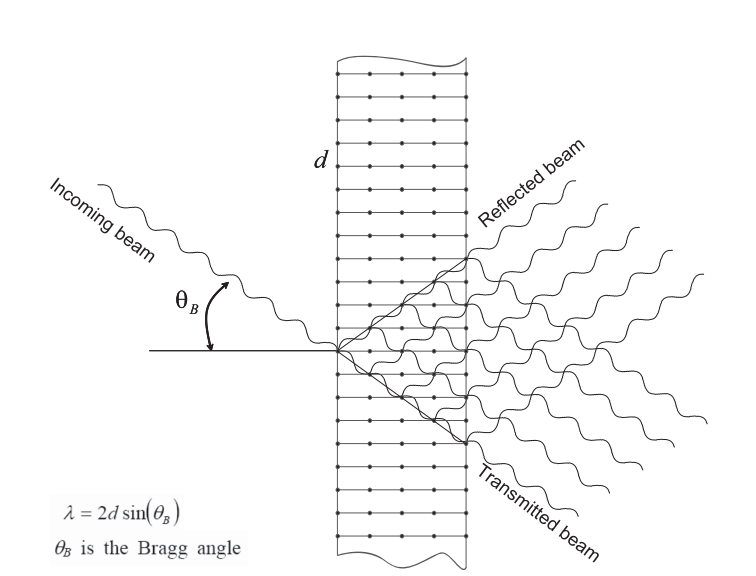
\includegraphics[scale=0.5]{Figures/braggscattering.png}
\caption{Bragg scattering off of a crystal lattice}
\label{fig:braggscattering}
\end{figure}

\subsection{Quantum Scattering Theory}
\label{sec:scatteringTheory}
 Starting with the assumption the Hamiltonian has the form of 
 \begin{equation}
 \mathcal{H} = \mathcal{H}_0+\mathcal{V} \,\,\,\,\, \mathcal{H}_0= \frac{\textbf{p}^2}{2m}
 \label{eq:hamiltonian}
 \end{equation}
The presence of the potential $\mathcal{V}$ causes the solution to be different than the free particle state 
$$\mathcal{H}_0\Ket{\Phi}=E\Ket{\Phi}$$

Therefore we are looking for solutions to the Schrödinger equation of the form \cite{sakurai}
\begin{equation}
\label{eq:schrodinger}
(\mathcal{H}_0+\mathcal{V})\Ket{\Psi} = E\Ket{\Psi} 
\end{equation} 
 A valid solution should have that $\Ket{\Psi}\rightarrow\Ket{\Phi}$ as $\mathcal{V}\rightarrow 0$. A solution that satisfies these requirements is known as the Lippmann-Schwinger equation. \cite{sakurai}
 \begin{equation}
 	\label{lippmanSchwinger}
 	\Ket{\Psi^{\pm}}=\Ket{\Phi}+\frac{1}{E-\mathcal{H}_0\pm i\epsilon}\mathcal{V}\Ket{\Psi^{\pm}} 
 \end{equation}
 Here the energy $E$ was made slightly complex with the addition of $\pm \epsilon$ to deal with the singular nature of the operator $1/(E-\mathcal{H}_0)$. It can easily be seen that the application of the operator $E-\mathcal{H}_0$ reduces (\ref{lippmanSchwinger}) to the desired solution (\ref{eq:schrodinger}) when neglecting the imaginary component. By taking the Lipmann-Schwinger equation to the position basis explicitly it can be represented as \cite{sakurai}
 \begin{equation}
 \label{eq:positionBasis}
 \Braket{\mbox{\boldmath$x$}|\Psi^{\pm}}=\Braket{\mbox{\boldmath$x$}|\Phi} -\frac{2m}{\hbar^2} \int d^3x^{'} \frac{e^{\pm ik\left|\mbox{\boldmath$x-x^{'}$}\right|}}{ 4\pi \left| \mbox{\boldmath$x-x^{'}$} \right|} \Braket{\mbox{\boldmath$x^{'}$}|\mathcal{V}|\Psi^{\pm}}
 \end{equation}
As our scattering potentials are a function of position only the assumption can be made that the potential is \textit{local} such that it is diagonal in the position representation. Specifically the potential satisfies the requirement that \cite{sakurai}
\begin{equation}
\label{eq:localPotential}
\braket{\mbox{\boldmath$x^{'}$}|\mathcal{V}|\mbox{\boldmath$x^{''}$}}=\mathcal{V}(\mbox{\boldmath$x$}^{'})\delta^{(3)}(\mbox{\boldmath$x^{'}$}-\mbox{\boldmath$x^{''}$})
\end{equation}

Utilizing this potential we obtain 
\begin{equation}
\label{eq:localPotentialResult}
\Braket{\mbox{\boldmath$x$}|\mathcal{V}|\Psi^{\pm}}=\int d^3x^{''} \braket{\mbox{\boldmath$x^{'}$}|\mathcal{V}|\mbox{\boldmath$x^{''}$}} \braket{\mbox{\boldmath$x^{''}$}|\Psi^{\pm}}=\mathcal{V}(\mbox{\boldmath$x^{'}$})\braket{\mbox{\boldmath$x^{'}$}|\Psi^{\pm}}
\end{equation}
With this result the Lippmann-Schwinger equation can be reduced to 
\begin{equation}
\label{eq:lippmannSchwingerLocal}
 \Braket{\mbox{\boldmath$x$}|\Psi^{\pm}}=\Braket{\mbox{\boldmath$x$}|\Phi} -\frac{2m}{\hbar^2} \int d^3x^{'} \frac{e^{\pm ik\left|\mbox{\boldmath$x-x^{'}$}\right|}}{ 4\pi \left| \mbox{\boldmath$x-x^{'}$} \right|} \mathcal{V}(\mbox{\boldmath$x{'}$})\Braket{\mbox{\boldmath$x^{'}$}|\Psi^{\pm}}
\end{equation}
Given that we are concerned with studying finite range scatters and that any observations that will be made outside the range of the potential due to the macroscopic nature of neutron detectors, the assumption can be made that $\left|\mbox{\boldmath$x$}\right| >>\left|\mbox{\boldmath$x^{'}$}\right|$. The finite range potential can be seen in fig(\ref{fig:finiteRangePotential}).
\begin{figure}[ht!]
\centering
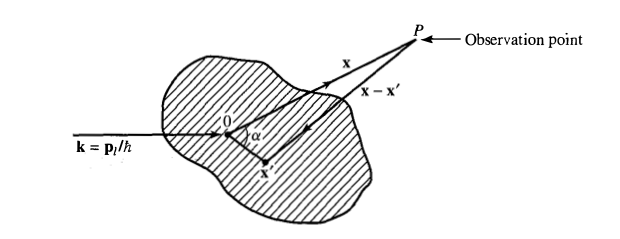
\includegraphics[scale=0.5]{Figures/scatteringObservation.png}
\caption{The finite range scattering potential. Any observations via detectors will be outside the range of the potential and therefore approximations can be made when evaluating (\ref{eq:lippmannSchwingerLocal}).}
\label{fig:finiteRangePotential}
\end{figure}

Keeping in mind this result we can define \cite{sakurai}
$$ r = \left| \mbox{\boldmath$x$} \right| $$
$$r^{'}=\left|\mbox{\boldmath$x^{'}$}\right|$$
$$\alpha = \angle(\mbox{\boldmath$x,x^{'}$})$$
$$\mbox{\boldmath$\hat{r}$} \equiv \frac{\mbox{\boldmath$x$}}{\left|\mbox{\boldmath$x$}\right|}$$

\begin{equation}
\label{eq:toObservation}
\left|\mbox{\boldmath$x-x^{'}$}\right| \approx r-\mbox{\boldmath$\hat{r}\cdot x^{'}$}
\end{equation}
\begin{equation}
\label{eq:propogationVector}
\mbox{\boldmath$k^{'}$} \equiv k\mbox{\boldmath$\hat{r}$}
\end{equation}

Utilizing equations (\ref{eq:toObservation},\ref{eq:propogationVector})
\begin{equation}
e^{\pm ik \left|\mbox{\boldmath$x-x^{'}$}\right|} \approx e^{\pm ikr}e^{\mp i \mbox{\boldmath$k^{'}\cdot x^{'}$}}
\label{eq:waveSimplification}
\end{equation}
For the distant $r$ at the observation point it is a useful approximation to say that 
\begin{equation}
\frac{1}{\left|\mbox{\boldmath$x-x^{'}$}\right|} \approx \frac{1}{r}
\end{equation}
Now replacing our incident generic wave with an incident plane wave $\Ket{\Phi}\rightarrow \Ket{\mbox{\boldmath$p$}}$ and using \mbox{\boldmath$k$} $\equiv \mbox{\boldmath$p_i$}/ \hbar$ to remove the $\hbar$'s from the expression.\cite{sakurai} We obtain for the first term in (\ref{eq:lippmannSchwingerLocal}) 
\begin{equation}
\Braket{\mbox{\boldmath$x$}|\mbox{\boldmath$k$}}=\int d^3k^{'} \Braket{\mbox{\boldmath$x$}|\mbox{\boldmath$k^{'}$}}\Braket{\mbox{\boldmath$k^{'}$}|\mbox{\boldmath$k$}}=\int d^3k^{'}  \Braket{\mbox{\boldmath$x$}|\mbox{\boldmath$k^{'}$}} \delta^{(3)}(\mbox{\boldmath$k^{'}-k$})=\frac{e^{i\mbox{\boldmath$k \cdot x$}}}{(2\pi)^{\frac{3}{2}}}
\label{eq:PlaneWave}
\end{equation}
Using this result in (\ref{eq:lippmannSchwingerLocal}) gives an expression for the scattered wave function at a relatively distant observation point for the positive Lippmann-Schwinger wavefunction. 
\begin{equation}
\label{eq:scatteredEquation}
\Braket{\mbox{\boldmath$x$}|\Psi^{+}} = \frac{1}{(2\pi)^{\frac{3}{2}}}\left(e^{i\mbox{\boldmath$k \cdot x$}} + \frac{e^{ikr}}{r}f(\mbox{\boldmath$k^{'},k$})\right)
\end{equation}
\begin{equation}
\label{eq:f}
f(\mbox{\boldmath$k^{'},k$})=-m\left(\frac{2\pi}{h}\right)^2\Braket{\mbox{\boldmath$k^{'}$}|\mathcal{V}|\Psi^{+}}
\end{equation}
It is very easy to see that the result wavefunction is a combination of the original incident plane-wave and an outgoing spherical wave with an amplitude described by (\ref{eq:f}). An obvious issue is that here scattering has only been treated for an incident plane-wave which is not a normalizable wavefunction. In reality to describe discrete particles such as neutrons wave packet solutions are used to describe the incident particles. However, provided the size of the wave packet is much larger than the range of the finite potential $\mathcal{V}$ it is sufficient to treat an incident packet as a plane-wave.  
\subsection{Differential Scattering Cross-Section}
The scattering cross section is an important parameter for experimental scattering physics. It relates the number of particles scattering into the solid angle $d\Omega$ per unit time to the number of incident particles into an infinitesimal element $d\sigma$ of area per unit time. We search for a relation between $d\Omega$ and $d\sigma$ which we term the differential cross section given by $d\sigma/d\Omega$.\cite{sakurai}
\begin{figure}[ht!]
\centering
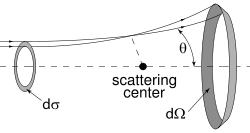
\includegraphics[scale=1.0]{Figures/scatteringCrossSection.png}
\caption{The differential cross section is the relationship between incident particles travelling through area $d\sigma$ to scattered particles crossing through the solid angle $d\Omega$. \cite{sakurai}}
\label{fig:scatteringCrossSection}
\end{figure}
Evidently the probability of an incident particle being within an area $d\sigma$ in time $dt$ while travelling with velocity $v$ is \cite{griffiths}
\begin{equation}
dP = \left|\Psi_i\right|^2 dV  = \left(\frac{1}{2\pi}\right)^3 (vdt)d\sigma
\label{eq:incidentCross}
\end{equation}

\begin{figure}[ht!]
\centering
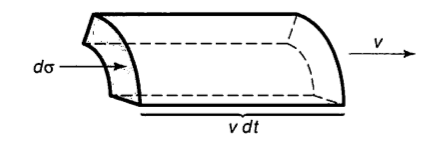
\includegraphics[scale=0.7]{Figures/incidentBeam.png}
\caption{The volume element $dV$ that a beam occupies passing through an area $d\sigma$ in time $dt$. \cite{griffiths}}
\label{fig:incidentBeam}
\end{figure}

Relating this probability to the probability of a particle being scattered into solid angle $d\Omega$ with equal velocity $v$ per unit time $dt$. 
\begin{equation}
\label{eq:scatteredCross}
dP=\left|\Psi_s\right|^2dV = \left(\frac{1}{2\pi}\right)^3 \frac{\left|f(\mbox{\boldmath$k^{'},k$})\right|^2}{r^2}(vdt)r^2 d\Omega
\end{equation}
Equations (\ref{eq:incidentCross}) and (\ref{eq:scatteredCross}) can be solved for the differential cross section 
\begin{equation}
\label{eq:differentialCrossSection}
\frac{d\sigma}{d\Omega}= \left|f(\mbox{\boldmath$k^{'},k$})\right|^2
\end{equation}

\subsection{Scattering Amplitude}
While equation (\ref{eq:f}) defines the magnitude of the outgoing spherical wave, it is defined implicitly in terms of the unknown ket $\Ket{\Psi^{+}}$. The solution to this problem in the case of sufficiently weak scatterers is to use the first Born approximation \cite{sakurai}
\begin{equation}
\label{eq:born}
\Braket{\mbox{\boldmath$x^{'}$}|\Psi^{+}} \rightarrow \Braket{\mbox{\boldmath$x^{'}$}| \Phi} = \frac{e^{i\mbox{\boldmath$k\cdot x^{'}$}}}{(2\pi)^{3/2}}
\end{equation}
Combining (\ref{eq:born}) and (\ref{eq:f}) results in the first-order Born amplitude \cite{sakurai}
\begin{equation}
\label{eq:firstOrderBorn}
f^{(1)}(\mbox{\boldmath$k^{'},k$}) = -\frac{m}{2\pi\hbar^2}\int d^3x^{'}e^{i(\mbox{\boldmath$k-k^{'}$})\cdot \mbox{\boldmath$x^{'}$}}\mathcal{V}(\mbox{\boldmath$x^{'}$})
\end{equation}
As the potentials that will be dealt with are spherically symmetrical, further approximations can be made utilizing $\mbox{\boldmath$q$} \equiv \mbox{\boldmath$k-k^{'}$}$ and $$\left|\mbox{\boldmath$k-k^{'}$}\right| \equiv  q = 2ksin \left( \frac{\theta}{2}\right)$$ as seen in fig(\ref{fig:scatteringAngle}) The spherical symmetry can be used to integrate explicitly the angular component of the scattering magnitude. \cite{sakurai}
\begin{figure}[ht!]
\centering
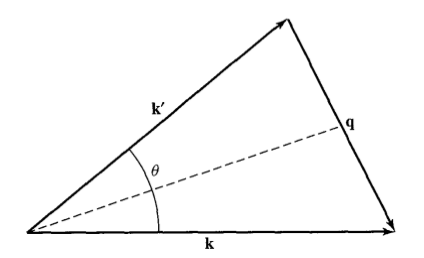
\includegraphics[scale=0.5]{Figures/scatteringAngle.png}
\caption{Scattering amplitude as a function of $\theta$ where $\mbox{\boldmath$q$}=\mbox{\boldmath$k-k^{'}$}$ \cite{sakurai}}
\label{fig:scatteringAngle}
\end{figure}
$$
f^{(1)}(\theta) =  -\frac{m}{2\pi\hbar^2} \int_{r=0}^{\infty} \int_{\phi=0}^{2\pi} \int_{\theta^{'}=0}^{\pi} e^{i \left| q \right| \left| r \right|cos(\theta^{'})}sin(\theta^{'})r^2 \mathcal{V}(r) d\theta^{'} d\phi dr
$$
\begin{equation}
\label{eq:bornAngular}
= -\frac{1}{2i}\frac{2m}{\hbar^2q} \int_{0}^{\infty} r\mathcal{V}(r)(e^{iqr}-e^{-iqr})dr = -\frac{2m}{\hbar^2}\frac{1}{q}\int_{0}^{\infty} r\mathcal{V}(r)sin(qr)dr
\end{equation}
Given a potential that has spherical symmetry it is now much more simple to calculate the scattering amplitude using (\ref{eq:bornAngular}).
\subsection{Neutron-nucleus Scattering}
Generally there are two interactions that an incident neutron on a material will experience, the interaction with the nucleus of the material atoms which is referred to as nuclear scattering and the scattering due to interactions with unpaired electrons and their magnetic moments which is known as magnetic scattering. In practice nuclear scattering is more common as it allows probing the structure of solids. 

Given the assumptions that an incoming neutron beam will be elastically scattered and that the nucleus is fixed, the scattering will depend on the potential $V(\mbox{\boldmath$r$})$ between the nucleus and neutron. As this interaction is due to the strong-force it is naturally occurring over a very short range, and is approximately zero at a distance of the order $\mbox{\boldmath$r$}=10^{-15}m$. As this is much shorter than the wavelength of thermal and cold neutrons which are used in almost all scattering experiments, the nucleus acts as a point scatterer. A neutron beam can be represented as a plane wave a wave function described by (\ref{eq:PlaneWave}) and the scattered wavefunction will take the form of (\ref{eq:scatteredEquation},\ref{eq:f}).

Due to the magnitude of the difference between the wavelength of the incident neutrons and the effective acting distance of the strong-force neutron-nucleus interaction and its approximate spherical symmetry it is an acceptable approximation to use the Fermi pseudo-potential \cite{waveguide}
\begin{equation}
\label{eq:FermiPseudoPotential}
\mathcal{V}(\mbox{\boldmath$x^{'}$}) = \frac{2\pi\hbar^2}{m}b\delta(\mbox{\boldmath$x^{'}$})
\end{equation}
 as a scattering potential. Where $b$ is known as the neutron scattering length and has units of meters. For the case of multiple nuclei the potential takes the form
 \begin{equation}
 \label{eq:MultipleNuclei}
 \mathcal{V}(\mbox{\boldmath$x^{'}$})  = \frac{2\pi\hbar^2}{m}\sum\limits_{j} b_j \delta(\mbox{\boldmath$x^{'}-x_j$})
 \end{equation}

Using the spherical approximate Born solution for the amplitude (\ref{eq:firstOrderBorn}) and the Fermi pseudo-potential the scattering amplitude can be found to be 
\begin{equation}
f^{(1)}(\theta) = -\int d^3x^{'}e^{i(\mbox{\boldmath$k-k^{'}$})\cdot \mbox{\boldmath$x^{'}$}}\sum\limits_{j} b_j \delta(\mbox{\boldmath$x^{'}-x_j$})=-\sum\limits_{j}b_j e^{i(\mbox{\boldmath$q \cdot x_j$})}
\label{eq:neutronScatteringAmplitude}
\end{equation}
And in the case of a single scatterer at the origin reducing to 
\begin{equation}
f^{(1)}(\theta)  = -b
\label{eq:neutronScatteringSingle}
\end{equation}
Therefore it can be seen that the completed neutron scattered wave form is
\begin{equation}
\label{eq:scatterNeutronWaveForm}
\Braket{\mbox{\boldmath$x$}|\Psi^{+}} = \frac{1}{(2\pi)^{\frac{3}{2}}}\left(e^{i\mbox{\boldmath$k \cdot x$}} - \sum\limits_{j}b_j e^{i(\mbox{\boldmath$q \cdot x_j$})}\frac{e^{ikr}}{r}\right)
\end{equation}

From this approximate solution it is evident that the only difference between individual scatterers is their neutron scattering length $b$. The value $b$ varies greatly among even neighbouring elements in the periodic table. Unfortunately the outlined theory is not strong enough to predict the scattering length and the parameters must be determined experimentally. Fig(\ref{fig:scatteringLength}) shows the scattering length for various elements of the periodic table.

\begin{figure}[ht!]
\centering
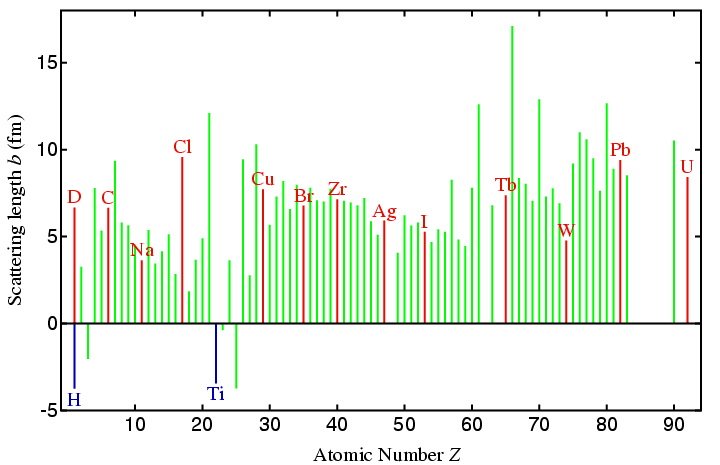
\includegraphics[scale=0.5]{Figures/neutronScatteringLength.png}
\caption{Neutron scattering lengths $b$ for the elements of the periodic table. \cite{scatteringlengths}}
\label{fig:scatteringLength}
\end{figure}

Inside a sufficiently large homogeneous material the Fermi pseudo-potential can be approximated to be 

\begin{equation}
 \mathcal{V}(\mbox{\boldmath$x^{'}$})  = \frac{2\pi\hbar^2}{m}\sum\limits_{j} b_j \delta(\mbox{\boldmath$x^{'}-x_{j}$}) \approx \frac{2\pi\hbar^2}{m}bN 
\label{eq:approxFermiPseudopotential}
\end{equation}

Where $N$ is the atom number density. 
\subsection{Neutron Optics}
As the neutron beam is a wavefunction many analogies from classical optics hold. The index of refraction is defined as the ratio of the speed of neutrons experiencing no potential to the speed of neutrons affected by a potential. Compared to light the form is familiar 
$$ n = \frac{c}{v} = \frac{K}{k}$$
Where from Schrödinger's equation
$$\nabla^2\Psi(\mbox{\boldmath$x$}) + \frac{2m}{\hbar^2}(E-\mathcal{V}(\mbox{\boldmath$x$}))\Psi(\mathbf{x}) = 0 $$ 
\begin{equation}
\label{eq:K}
K^2 = \frac{2m}{\hbar^2}(E-\mathcal{V}(\mbox{\boldmath$x$}))
\end{equation}
\begin{equation}
\label{eq:NinPotential}
n(\mbox{\boldmath$x$}) = \frac{K}{k} = \sqrt{\frac{E-\mathcal{V}(\mbox{\boldmath$x$})}{E}}=\sqrt{1-\frac{\mathcal{V}(\mbox{\boldmath$x$})}{E}}
\end{equation}
Given that the neutron scattering potentials are described by (\ref{eq:approxFermiPseudopotential}) the index of refraction can be approximated to \cite{waveguide}
\begin{equation}
n(\mbox{\boldmath$x$}) = \sqrt{1-\frac{\frac{2\pi\hbar^2}{m}bN}{E}}= \sqrt{1 - \frac{4\pi bN}{k^2}}
\label{eq:indexofrefraction}
\end{equation}

In the case of magnetic materials the magnetic potential
\begin{equation*}
\mathcal{V}_{mag}(\mbox{\boldmath$x$})=-\mbox{\boldmath$u \cdot B_{eff}$}
\end{equation*}
 must be accounted for. This results in an index of refraction for magnetic materials such as Fe,Ni and Co of 
\begin{equation}
n_{\pm}(\mbox{\boldmath$x$})= \sqrt{1-\frac{\frac{2\pi\hbar^2}{m}bN \mp \mbox{\boldmath$u \cdot B_{eff}$}}{E}}
\label{eq:nucleurIndexofRefraction}
\end{equation}
\subsection{Neutron in Material Phase-Shift}
The phase shift due to a perturbing potential is given by \cite{green_2}
\begin{equation}
\phi = \frac{1}{\hbar}\int  \mathbf{p}\cdot \mathbf{dl} = \int \mathbf{K}\cdot d\mathbf{l}= \int \mathbf{nk}\cdot \mathbf{dl}
\label{eq:phase_shift}
\end{equation}
Where $\mathbf{n}$ is the neutron index of refraction and $\mathbf{k}$ is the neutron wave vector. Under the assumption that $\mathbf{n}$ is isotropic and that the perturbation that creates $\mathbf{n}$ does not shift the path to a large degree, the phase difference between two optical paths may be written as
\begin{equation}
\delta\phi = \int (n_1-n_2)\mathbf{k}\cdot \mathbf{dl} = Nb\lambda D
\label{eq:phase_shift_full}
\end{equation}
Where $D$ is the thickness of the material the neutron beam travels through.  

\subsection{Mach-Zehnder Interferometer}

The MZ utilizes a half-mirror to split the incoming electromagnetic wave and the resultant two beam paths are refocused on a second beam-splitter. The two interfered waveforms exit the second beam-splitter and are incident on two detectors that can be visualized as Detector 1 \& 2 in fig(\ref{mach-zehnder}),

\begin{figure}[ht!]
\centering
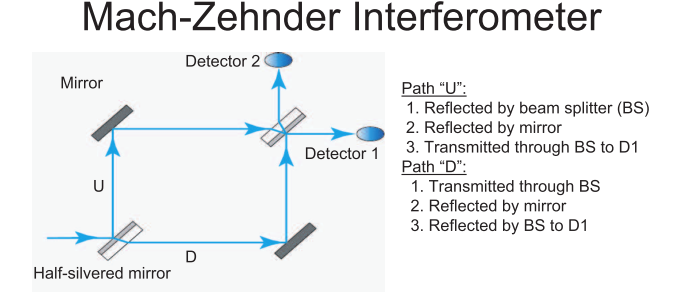
\includegraphics[scale=0.65]{Figures/mach-zender.png}
\caption{The Mach-Zehnder interferometer. \cite{dimaThesis}}
\label{mach-zehnder}
\end{figure}

As reflection results in a phase shift of $\pi$ and assuming transmission through the half-mirrors results in a phase shift of $\delta$, we easily calculate the phase differences of the two paths at the two detectors. At detector 1 and path $U$ there is a total of two reflections and a single transmission which results in a phase shift of $2\pi+\delta$. Similarly for path $D$ the phase shift is also $2\pi + \delta$. Therefore at detector 1 there is constructive interference. At detector 2 path $U$ has a phase of $2\pi + 2\delta$ and path $D$ has a phase of $\pi + 2\delta$. Therefore at detector 2 there is destructive interference.\cite{dimaThesis}

\subsection{Three Blade Perfect Crystal Neutron Interferometer}
When inside the neutron interferometer it is useful to analyse the wavefunction as the sum of the two possible neutron paths which will be referred to as path one $\Psi_0 = \Ket{I}$ and path two $\Ket{II}$. The wavefunction inside the interferometer can be represented by\cite{dimaThesis} 
\begin{equation*}
\Psi = C_1e^{i\phi_1}\Ket{I} + C_2e^{i\phi_2}\Ket{II}
\end{equation*}
Where $\phi_i$ are the phase of each component and $C_i$ are the amplitudes of each component. Representing the amplitude of a Bragg transmitted wave as $t$ and the reflected amplitude as $r$, where $|r|^2+|t|^2 = 1$. 

The wavefunctions can be traced through the interferometer. Consider an initial neutron with wavefunction $\Ket{I}$ is incident on the first blade of the neutron interferometer. The resultant wavefunction is 
$$ te^{i\phi_{1_1}}\Ket{I} + re^{i\phi_{2_1}}\Ket{II}$$
This wavefunction is than incident on the second blade interferometer. Discarding the transmitted waves as they exit the interferometer, the resultant wavefunction is 
$$rte^{i\phi_{1_2}}\Ket{I} + rre^{i\phi_{2_2}}\Ket{II}$$
At the third and final blade, the geometry of the wave splitting superimposes path one and two onto each-other the two resultant beams are incident on two detectors, the upper detector known as the $O$ detector upon which the $O$ beam is incident and the lower which is known as the $H$ detector upon which the $H$ beam is incident. The resultant wave functions are 
\begin{equation}
\Ket{\Psi_O} = (rrte^{i\phi_1}+trre^{i\phi_2}) \Ket{I} \,\,\,\,\,\, \Ket{\Psi_H} = (trte^{i\phi_1}+rrre^{i\phi_2})\Ket{II}
\label{eq:beams}
\end{equation}
This results in an intensity at the $O$ detector of\cite{dimaThesis}
\begin{equation}
I_O \propto P(O|\Delta\phi) = \Braket{\Psi_O | \Psi_O} = |r|^4|t|^2(1+cos(\phi_1-\phi_2) = A(1+cos(\Delta\phi))
\label{eq:obeamintensity}
\end{equation} 
Where $A=|r|^4|t|^2$ and $\Delta\phi = \phi_1-\phi_2$. The resultant intensity for the $H$ beam is therefore 
\begin{equation}
I_H \propto P(H|\Delta\phi) = \Braket{\Psi_H | \Psi_H} = (|t|^4|r|^2 + |r|^6)-|r|^4|t|^2(cos(\phi_1-\phi_2)) = B - Acos(\Delta\phi)
\label{eq:hbeamintensity}
\end{equation}
Where $B=|t|^4|r|^2 + |r|^6$. 

The contrast of the neutron interferometer detectors is defined as 
\begin{equation}
C = \frac{\text{max}(I)-\text{min}(I)}{\text{max}(I)+\text{min}(I)}
\label{eq:contrastdefinition}
\end{equation}
Clearly than the contrast of the $O$ beam will be $1$ in the ideal case. However, the contrast of the $H$ beam will depend on the size of the reflection coefficient $r$. 
\begin{equation}
C_O = 1 \,\,\,\,\,\, C_H = \frac{|r|^4|t|^2}{|t|^4|r|^2+|r|^6}
\label{eq:contrasts}
\end{equation}
In (\ref{eq:hbeamintensity},\ref{eq:obeamintensity}) the intensities account for the loss of neutrons due to the transmitted neutrons in the second blade which exit the interferometer. This is apparent as 
$I_O+I_H \neq 1$. If the assumption is made that information is not lost with the exit of those neutrons the intensities can be reformulated by treating the second blades as ideal mirrors resulting in the new intensity formulation of\cite{dimaThesis}
\begin{equation}
I_O \propto P(O|\Delta\phi) = 2|rt|^2(1+cos(\Delta\phi)) \,\,\,\,\, I_H \propto P(H|\Delta\phi) = (|r|^4+|t|^4)-2|rt|^2cos(\Delta\phi)
\label{eq:normalizedIntensities}
\end{equation}
This revised intensity equation satisfies the property that $P(O|\Delta\phi)+P(H|\Delta\phi) = 1$. 
\subsection{Phase Flag}
\label{sec:phaseflag}
Utilizing the phase shift due to the neutron beam passing through a perturbing potential it is possible to analyse materials via the induced phase shift. 

\begin{figure}[ht!]
\centering
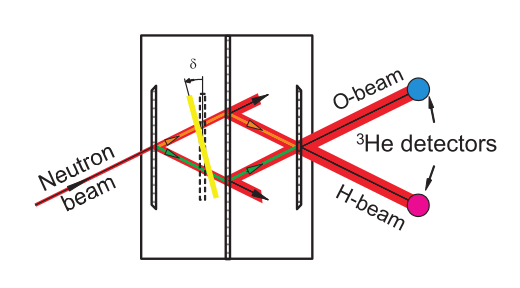
\includegraphics[scale=0.7]{Figures/phase_flag.png}
\caption{Neutron interferometer with a phase flag \cite{dimaThesis} }
\label{fig:phaseflag}
\end{figure}

As seen in fig(\ref{fig:phaseflag}) the two paths will pass through the phase flag. Providing the angle of the phase flag $\delta$ is not equal to zero the paths $D_1$ and $D_2$ will accrue a phase shift due to the different path lengths inside the material. The path lengths of the up and down beams are given by 
\begin{equation}
d_1 = \frac{D}{cos(\theta_B -\delta)} \,\,\,\,\, d_2 = \frac{D}{cos(\theta_B +\delta)}
\label{eq:phase_path_lengths}
\end{equation}
Where $D$ is the thickness of the phase flag, $\theta_B$ is the scattering Bragg angle of the two neutron beams relative to the horizontal, and $\delta$ is the angle of the phase flag relative to the vertical. Using these paths lengths and (\ref{eq:phase_shift_full}) the phase shift along each path are 
\begin{equation*}
\delta\phi_1 = \frac{Nb\lambda D}{ cos(\theta_B -\delta)} \,\,\,\,\, \delta\phi_2 = \frac{Nb\lambda D}{ cos(\theta_B +\delta)}
\end{equation*}
Which gives a relative phase between the two beams of 
$$\Delta\phi = Nb\lambda D \left(\frac{1}{cos(\theta_B -\delta)} - \frac{1}{cos(\theta_B +\delta)}\right) = $$
\begin{equation}
=-2NbD\lambda \frac{sin(\theta_B)sin(\delta)}{cos^2(\theta_B)-sin^2(\delta)} \approx (CONSTANT)\times \delta = C\delta
\label{eq:relative_phase}
\end{equation}
It should be noted that as (\ref{eq:relative_phase}) relies on a small angle approximation, the result only hold for approximately $\delta=0..\pi/10$. Due to this restriction of phase flag angles to have full control of the phase we require that
\begin{equation}
C\times  \geq \frac{2\pi}{\frac{\pi}{10}} = 20
\
\end{equation}
Using this result the intensity at the $O$ and $H$ detectors become 
\begin{equation}
I_O \propto  P(O|\Delta\phi,\delta) = A(1+cos(\Delta\phi)+C\delta) \,\,\,\,\, I_H \propto P(H|\Delta\phi,\delta) = B - Acos(\Delta\phi+C\delta)
\label{eq:intensities_phase_shift}
\end{equation}
The contrast of the neutron interferometer is a function of the phase flag angle and measured intensities at the neutron detectors\cite{noise_neutron}
\begin{equation}
C_0 = \frac{\text{max}[D_0(\delta)] - \text{min}[D_0(\delta)]}{\text{max}[D_0(\delta)] + \text{min}[D_0(\delta)]}
\label{eq:contrast}
\end{equation}
Where $D_0$ is the detected neutron intensity at the $O$ detector. Similarly to the case without a phase flag, the maximum contrast for the $O$ beam is $1$ and the H beam depends on the coefficient $r$. 
\subsection{Neutron Wave Guides}
\label{sec:waveguide}
As neutrons are a wave, similarly to light the obey Snell's Law 
\begin{equation}
n_1sin(\theta_1) = n_2sin(\theta_2)
\label{eq:snellslaw}
\end{equation}
Total reflection will occur when 
$$sin(\theta_2)= \frac{n_1}{n_2}sin(\theta_1)\le 0 \,\,\,\,\, \{\forall  \theta \in \mathcal{R}: 0<\theta<\pi\}$$
As $max(sin(\theta_1))=1$ occur when $\theta_1=\frac{\pi}{2}$, using (\ref{eq:indexofrefraction}) the condition for total reflection in air where $n_1\approx1$ is  
\begin{equation}
V(x)> E_\perp
\label{eq:interalreflection}
\end{equation}
Therefore given a material with large enough values for $N$ and $b$ it is possible to design a waveguide for neutrons as they will simply reflect back and forth inside the guide as seen in fig(\ref{fig:waveguide}).  

\begin{figure}[ht!]
\centering
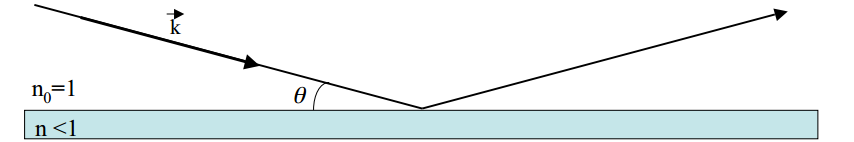
\includegraphics[width=\textwidth]{Figures/waveguide.png}
\caption{Neutron waveguide under the assumption that there is no Bragg scattering and the absorption is negligible \cite{waveguide} }
\label{fig:waveguide}
\end{figure}